% IEEE conference paper. Overleaf: upload the whole paper/ folder AND literature/references.bib
% (or keep the relative path below if you upload the repo root).
\documentclass[conference]{IEEEtran}
\IEEEoverridecommandlockouts

\usepackage{iftex}
\ifTUTeX
  \usepackage{fontspec}
  \setmainfont{texgyretermes}[
    Extension=.otf,
    UprightFont=*-regular,
    BoldFont=*-bold,
    ItalicFont=*-italic,
    BoldItalicFont=*-bolditalic
  ]
  \setsansfont{texgyreheros}[
    Extension=.otf,
    UprightFont=*-regular,
    BoldFont=*-bold,
    ItalicFont=*-italic,
    BoldItalicFont=*-bolditalic,
    Scale=MatchLowercase
  ]
  \setmonofont{texgyrecursor}[
    Extension=.otf,
    UprightFont=*-regular,
    BoldFont=*-bold,
    ItalicFont=*-italic,
    BoldItalicFont=*-bolditalic,
    Scale=0.86
  ]
\else
  \usepackage[T1]{fontenc}
  \usepackage[utf8]{inputenc}
\fi

\usepackage{cite}
\usepackage{amsmath,amssymb}
\usepackage{graphicx}
\usepackage{booktabs}
\usepackage{array}
\usepackage{siunitx}
\usepackage{xcolor}
\usepackage{xurl}
\usepackage{microtype}
\usepackage[hidelinks]{hyperref}

\graphicspath{{figures/}}

\begin{document}

\title{Flutter vs.\ Native Android for On-Device Inference: An Empirical Benchmark on Entry-Tier Hardware}

\author{
\IEEEauthorblockN{Hassaan Khalid}
\IEEEauthorblockA{\textit{Department of Software Engineering}\\
\textit{University of Sargodha}\\
Sargodha, Pakistan\\
hassaankhalid225@gmail.com}
}

\maketitle

\begin{abstract}
On-device deep learning inference is increasingly integrated into consumer smartphone applications to guarantee low latency, user privacy, and offline functionality. While cross-platform frameworks---predominantly Google Flutter---dominate modern mobile application engineering, developers face an empirical vacuum regarding whether cross-platform abstractions degrade deep learning performance compared to native implementations. This paper presents the first controlled, full-factorial benchmark comparing Flutter and Native Android implementations of identical on-device inference workloads using Google LiteRT (formerly TensorFlow Lite). Evaluating three diverse model architectures (MobileNetV3-Large, EfficientDet-Lite0, MobileBERT-QA) across single-precision floating-point (FP32) and integer quantization (INT8), three execution delegates (multi-threaded CPU with XNNPACK, GPU, and NNAPI), and eight independent sessions per configuration, we isolate and decompose latency across data preprocessing, language-boundary foreign function interface (FFI) marshalling, native kernel execution, and postprocessing. Our empirical results demonstrate that pure kernel inference latency exhibits complete parity between Flutter and Native Android. The user-perceived end-to-end latency differential is overwhelmingly driven by data ingestion and image preprocessing in pure Dart rather than the runtime inference engine. Furthermore, while Flutter incurs fixed baseline memory and cold-start startup premiums due to its embedded virtual machine, incremental memory allocated per model arena remains equivalent. We synthesize our findings into an evidence-based decision matrix, identifying actionable thresholds for when standard Flutter is completely sufficient and when native preprocessing optimizations are justified.
\end{abstract}

\begin{IEEEkeywords}
on-device inference, edge AI, Flutter, cross-platform development, LiteRT, mobile performance, benchmarking, software engineering
\end{IEEEkeywords}

\section{Introduction}\label{sec:intro}

Deep learning models are increasingly deployed directly on mobile edge devices to deliver low-latency, privacy-preserving, and offline-capable intelligence~\cite{xu2019first,lane2015early}. Consumer smartphone applications routinely embed neural networks for camera image enhancement, real-time object detection, biometric authentication, and natural language understanding~\cite{almeida2021smart,wu2019machine}. However, executing complex deep neural networks within the strict thermal, battery, and memory envelopes of mobile handsets presents acute systems engineering challenges~\cite{lane2016deepx,banbury2021benchmarking}.

Concurrently, multi-platform mobile application development frameworks have achieved widespread industrial adoption~\cite{biornhansen2018survey}. Google's Flutter framework, in particular, has emerged as a dominant stack for modern mobile applications, enabling software teams to target Android and iOS from a single Dart codebase. Unlike legacy hybrid frameworks that rely on interpreted JavaScript bridges or WebView wrappers~\cite{ciman2017empirical,delia2015performance}, Flutter compiles Dart ahead-of-time (AOT) to native ARM machine code and renders interfaces directly via its dedicated graphics engine~\cite{biornhansen2020empirical}.

Despite the widespread adoption of both mobile deep learning and Flutter, a critical architectural gap persists in software engineering practice. On-device inference engines---chiefly Google LiteRT (formerly TensorFlow Lite)---are compiled native C/C++ runtimes. When a Flutter application performs inference, execution must cross a foreign function interface (Dart FFI) boundary. Furthermore, typical production Flutter developers perform data ingestion and preprocessing (such as JPEG image decoding, bilinear resizing, and tensor layout normalization) in pure Dart rather than platform-native code. Developers currently possess no empirical, statistically rigorous evidence quantifying the latency, memory, CPU, and energy costs introduced by this cross-platform software layer. Consequently, architectural decisions between cross-platform and native mobile stacks are guided by anecdotal claims.

Prior mobile machine learning benchmarking efforts, such as AI Benchmark~\cite{ignatov2018ai,ignatov2019ai}, MLPerf Mobile~\cite{reddi2022mlperfmobile}, and library comparative studies~\cite{zhang2022comprehensive,luo2020comparison}, focus almost exclusively on silicon accelerators (CPUs, GPUs, and NPUs) and native C++ runtime engines. These benchmarks evaluate standalone native binaries, deliberately abstracting away the application software frameworks in which deep learning models are actually integrated. Conversely, existing empirical studies of cross-platform performance~\cite{biornhansen2020empirical,willocx2016comparing} evaluate synthetic microbenchmarks or generic UI navigation, omitting high-throughput tensor operations and hardware-delegated inference workloads.

To resolve this empirical blind spot, this paper presents a controlled, full-factorial benchmark study comparing Flutter and Native Android implementations of identical on-device deep learning workloads. By enforcing strict parity---holding model binaries, LiteRT runtime versions, hardware execution delegates, CPU thread configurations, and input sequences identical across both platforms---we isolate and quantify the exact overheads introduced by Flutter.

Our empirical investigation addresses five formal research questions:
\begin{enumerate}
    \item[\textbf{RQ1:}] \textit{Inference Latency.} Is there a statistically or practically significant difference in pure runtime inference latency ($\text{inference\_native\_ms}$) between Flutter and native Android when running identical LiteRT models and delegates?
    \item[\textbf{RQ2:}] \textit{End-to-End Latency Decomposition.} What is the latency discrepancy across the full input-to-result pipeline, and which stage (preprocessing, boundary marshalling, inference, or postprocessing) drives the differential?
    \item[\textbf{RQ3:}] \textit{Resource Utilization.} Does Flutter incur measurable premiums in peak memory consumption (proportional set size, PSS), CPU utilization, or battery drain under continuous inference workloads?
    \item[\textbf{RQ4:}] \textit{Interaction Effects.} How do model scale, precision format (FP32 vs.\ INT8), hardware acceleration delegate (CPU, GPU, NNAPI), and device hardware tiers interact with the cross-platform performance gap?
    \item[\textbf{RQ5:}] \textit{Application Footprint and Startup.} What are the relative penalties in cold-start latency to first inference and packaged application binary size?
\end{enumerate}

This paper provides four primary contributions:
\begin{itemize}
    \item \textbf{C1: Open-Source Parity-Checked Benchmark Suite.} We release open-source Flutter and Android Native benchmark applications implementing an identical execution contract, validated with cryptographic model verification and automated JSONL output validation.
    \item \textbf{C2: Controlled Empirical Characterization.} We execute a multi-tier study across 3 model architectures (MobileNetV3-Large, EfficientDet-Lite0, MobileBERT-QA), 2 numerical precisions (FP32, INT8), 3 execution delegates (CPU/XNNPACK, GPU, NNAPI), and multiple physical smartphone hardware tiers.
    \item \textbf{C3: Pipeline Overhead Decomposition.} We decompose end-to-end latency into data preprocessing, language boundary crossing, kernel invoke execution, and output postprocessing, exposing precisely where execution overheads originate.
    \item \textbf{C4: Evidence-Based Practitioner Guidelines.} We synthesize empirical findings into a structured decision matrix, providing mobile software architects with actionable thresholds for when Flutter is sufficient and when native implementation is justified.
\end{itemize}

The remainder of this paper is structured as follows. Section~\ref{sec:related} reviews related work in mobile deep learning and cross-platform benchmarking. Section~\ref{sec:method} details our experimental methodology, harness contracts, and statistical framework. Section~\ref{sec:results} presents our empirical results corresponding to RQ1--RQ5. Section~\ref{sec:discussion} discusses implications and provides engineering guidelines. Section~\ref{sec:threats} examines threats to validity, and Section~\ref{sec:conclusion} concludes the paper.

\section{Related Work}\label{sec:related}

\subsection{On-Device Deep Learning Benchmarking}
Early mobile AI measurements established the extreme performance diversity of smartphone accelerators. Ignatov et al.~\cite{ignatov2018ai,ignatov2019ai} introduced AI Benchmark across Android handsets, exposing wide latency disparities across CPU, GPU, and DSP/NPU backends. MLPerf Mobile~\cite{reddi2020mlperf,reddi2022mlperfmobile} standardized open-source accuracy and latency rules for edge vision and NLP models. Measuring in-the-wild deployment, Xu et al.~\cite{xu2019first} mined $16{,}500$ top Android apps and identified $211$ deep learning apps, noting rapid growth in embedded vision models such as MobileNet and SSD. Almeida et al.~\cite{almeida2021smart} compared device tiers and observed low-end and mid-tier phones running on average $3.4\times$ and $1.51\times$ slower than flagship silicon, showing non-linear FLOP-to-latency behavior driven by thermal throttling, scheduler policies, and excessive CPU thread contention. Recent benchmarks extend these measurements to generative mobile workloads, including MobileAIBench~\cite{murthy2024mobileaibench} and lm-Meter~\cite{wang2025lmmeter}, profiling end-to-end latency and memory dynamics of on-device language and multimodal models inside native C++/Android harnesses.

\subsection{Cross-Platform Mobile Framework Performance}
Bi{\o}rn-Hansen et al.~\cite{biornhansen2019survey} classified cross-platform architectures into WebView hybrids, JavaScript bridges, and natively compiled toolkits. Earlier comparisons by Willocx et al.~\cite{willocx2016comparing} and Del{\'\i}a et al.~\cite{delia2015multi} measured cold-launch delays and synthetic compute overheads across early hybrid stacks, while Ciman and Gaggi~\cite{ciman2017empirical} and Horn et al.~\cite{horn2023native} quantified persistent frame and energy costs relative to native Android. Focusing on modern AOT-compiled UI toolkits, Bi{\o}rn-Hansen et al.~\cite{biornhansen2020empirical} showed that Flutter approaches native UI frame responsiveness at the cost of higher memory consumption from the Dart VM and its Skia rendering layer; subsequent Flutter releases have migrated rendering from Skia to Impeller~\cite{flutterimpeller2025} (Vulkan on Android API~29+, OpenGL ES fallback on API~$\le 28$). Nanavati et al.~\cite{nanavati2024critical} further examined Flutter runtime profiling and memory tuning for UI-bound applications.

\subsection{Mobile Runtimes, Quantization, and Benchmark Rigor}
Inference efficiency depends strongly on native library implementation and numerical precision. Zhang et al.~\cite{zhang2022comprehensive} benchmarked six mobile engines across 15 models and 10 devices, finding that engine choice swings average latency by $7.4\times$ overall ($8.7\times$ CPU, $6.0\times$ GPU, and up to $54.3\times$ worst-case) while INT8 quantization delivers $0.8\text{--}3.0\times$ speedups; Luo et al.~\cite{luo2020comparison} similarly highlighted operator-coverage fragility across delegates. Jacob et al.~\cite{jacob2018quantization} formalized integer-only quantization to cut parameter footprints $4\times$ and accelerate SIMD hardware, yet delegation gains remain bounded by shader initialization and copy costs. Methodologically, Georges et al.~\cite{georges2007statistically} and Barrett et al.~\cite{barrett2017virtual} showed that managed-runtime benchmarks require separating warm-up transients from steady-state measurements, motivating Cliff's~$\delta$~\cite{cliff1993dominance} non-parametric dominance effects, bootstrap intervals, and Holm--Bonferroni family-wise control~\cite{holm1979simple}.

\subsection{Combined Research Gap}\label{subsec:gap}
Prior literature remains bifurcated across two silos. Machine learning benchmarks~\cite{ignatov2019ai,reddi2022mlperfmobile,zhang2022comprehensive,wang2025lmmeter} isolate C++ engines from host UI application frameworks, whereas cross-platform studies~\cite{biornhansen2020empirical,horn2023native,nanavati2024critical} test scrolling lists or synthetic loops without neural networks, delegates, or quantization. Consequently, no prior work isolates how a modern Flutter stack alters every pipeline stage---pure-Dart preprocessing, FFI marshalling, upstream dependency drift, and heap vs.\ \texttt{mmap} model loading---relative to idiomatic native Android under identical pinned models. Our protocol addresses this combined gap on entry-tier hardware using warm-up isolation, non-parametric equivalence tests, and session-level aggregation.

\section{Methodology}\label{sec:method}

To rigorously evaluate the performance characteristics of on-device deep learning inference across cross-platform and native stacks, we design a full-factorial, controlled empirical benchmark following pre-registered hypotheses and established systems evaluation standards~\cite{georges2007statistically,barrett2017virtual}.

\subsection{Experimental Design and Factors}
Our benchmark evaluates five controlled independent experimental factors, summarized in Table~\ref{tab:factors}:
\begin{enumerate}
    \item \textbf{Platform ($P$):} Flutter (Dart Ahead-Of-Time compiled) and Android Native (Kotlin compiled with R8 full-mode shrinking).
    \item \textbf{Model ($M$):} Three standard edge deep learning architectures spanning computer vision and natural language processing: MobileNetV3-Large~\cite{howard2019searching}, EfficientDet-Lite0~\cite{tan2020efficientdet}, and MobileBERT-QA~\cite{sun2020mobilebert}.
    \item \textbf{Precision ($Q$):} 32-bit floating-point (FP32) and full 8-bit integer post-training quantization (INT8)~\cite{jacob2018quantization}.
    \item \textbf{Hardware Delegate ($D$):} CPU multi-threading (4 threads with XNNPACK kernel acceleration), mobile GPU (OpenCL/OpenGL compute shaders), and Android Neural Networks API (NNAPI).
    \item \textbf{Device Tier ($T$):} Physical handsets spanning entry-level, mid-range, and flagship hardware profiles.
\end{enumerate}

\begin{table}[t]
\caption{Full-Factorial Experimental Design Matrix}
\label{tab:factors}
\centering
\begin{tabular}{ll}
\toprule
\textbf{Factor} & \textbf{Evaluated Levels} \\
\midrule
Platform & Flutter (Dart 3.12.2), Android Native (Kotlin 1.9.24) \\
Models & MobileNetV3-Large, EfficientDet-Lite0, MobileBERT-QA \\
Tasks & Image Classification, Object Detection, SQuAD 1.1 QA \\
Precision & FP32 (single precision), INT8 (quantized) \\
Delegates & CPU (4 threads, XNNPACK), GPU, NNAPI \\
Sessions & 8 independent sessions per configuration \\
Iterations & 20 warm-up + 100 measured per session \\
Canonical Inputs & 50 standardized images, 50 standardized text pairs \\
\bottomrule
\end{tabular}
\end{table}

\subsection{Benchmark Applications and Parity Contract}
Ensuring strict parity between cross-platform and native code is essential to guarantee that measured differentials reflect framework overhead rather than implementation divergence. Both benchmark applications strictly adhere to the \textit{Harness Contract}:
\begin{itemize}
    \item \textbf{Identical Runtime Engine:} Both applications link against Google LiteRT 2.16.1 (ADR-0002, ADR-0008). Flutter binds to the native shared C library via Dart FFI (`tflite\_flutter`), while Android Native binds via JNI.
    \item \textbf{Cryptographic Model Verification:} Model flatbuffer files (`*.tflite`) are pre-registered with cryptographic SHA-256 digests in `models/manifest.yaml`. At application initialization, both apps compute the runtime digest of the asset binary and abort execution if any hash discrepancy exists.
    \item \textbf{Standardized Input Sequence:} Both applications bundle identical asset sets (50 vision JPEGs and 50 text question/context pairs), processed in identical deterministic sequential order.
    \item \textbf{Realistic Developer Path:} In adherence to real-world software engineering practices, Flutter performs input image decoding and bilinear resizing using the pure Dart `image` package, representing typical Flutter application architecture. Android Native uses Android framework bitmap decoding.
    \item \textbf{Timed Region Isolation:} In accordance with contract specifications, no logging, disk I/O, garbage collection triggers, or UI allocations occur within the measured pipeline timestamps $t_0 \dots t_3$. Measurement records are buffered in heap memory and flushed to disk asynchronously after configuration completion.
    \item \textbf{Release Optimization:} All measurements are obtained exclusively from release-mode binaries (`flutter build apk --release` and Android R8-optimized release APKs). Debug builds (which employ JIT compilation) are strictly excluded.
\end{itemize}

\subsection{Pipeline Stage Definitions and Metric Formalism}
To isolate the precise origin of cross-platform overhead, we instrument each iteration across four discrete timestamps:
\begin{equation}
t_0 \xrightarrow{\text{preprocess}} t_1 \xrightarrow{\text{invoke}} t_2 \xrightarrow{\text{postprocess}} t_3
\end{equation}
where $t_0$ marks the availability of the raw asset in memory, $t_1$ marks input tensor buffer completion, $t_2$ marks the completion of the runtime `run()` invocation, and $t_3$ marks the production of the typed result object.

The individual latency metrics are formally defined as:
\begin{align}
\text{preprocess\_ms} &= \frac{t_1 - t_0}{10^6} \quad (\text{ms}) \\
\text{inference\_ms} &= \frac{t_2 - t_1}{10^6} \quad (\text{ms}) \\
\text{postprocess\_ms} &= \frac{t_3 - t_2}{10^6} \quad (\text{ms}) \\
\text{end\_to\_end\_ms} &= \frac{t_3 - t_0}{10^6} \quad (\text{ms})
\end{align}

\textbf{Boundary Overhead Measurement (ADR-0006):} The total invocation latency ($\text{inference\_ms}$) perceived by application code wraps input buffer copying, foreign function call transitions, kernel execution, and output buffer extraction. To isolate the pure kernel inference time, we interrogate the runtime's internal invoke timer:
\begin{equation}
\text{inference\_native\_ms} = \begin{cases}
\frac{\text{lastNativeInferenceDurationMicroSeconds}}{1000} & \text{(Flutter)} \\[4pt]
\frac{\text{lastNativeInferenceDurationNanoseconds}}{10^6} & \text{(Native)}
\end{cases}
\end{equation}
We derive the language-boundary marshalling overhead directly as:
\begin{equation}
\text{boundary\_overhead\_ms} = \text{inference\_ms} - \text{inference\_native\_ms}
\end{equation}
A timer residual check $\text{timer\_residual\_ms} = \text{end\_to\_end\_ms} - (\text{pre} + \text{inf} + \text{post})$ is monitored to verify timestamp continuity.

\textbf{System Resource Metrics:} Total memory consumption is recorded as Proportional Set Size ($\text{pss\_mb}$) via Android's `ActivityManager.getProcessMemoryInfo()`. Process CPU utilization ($\text{cpu\_pct}$) is computed via user and system execution time deltas in `/proc/self/stat`. Thermal throttling states ($\text{thermal\_status}$) are tracked via `PowerManager.getCurrentThermalStatus()`.

\begin{table*}[t]
\caption{Model Registry and Cryptographic Integrity Specifications}
\label{tab:models}
\centering
\begin{tabular}{lllllll}
\toprule
\textbf{Model ID} & \textbf{Task} & \textbf{Input Shape} & \textbf{Precision} & \textbf{Size (MB)} & \textbf{SHA-256 Checksum} & \textbf{Source Reference} \\
\midrule
mobilenetv3\_large & Classification & $[1, 224, 224, 3]$ & FP32 & 21.89 & \texttt{f924c190e9112c7db6630ab522c8fb2972be408180d2d72b8038e1a2340b2266} & Howard et al.~\cite{howard2019searching} \\
mobilenetv3\_large & Classification & $[1, 224, 224, 3]$ & INT8 & 5.67 & \texttt{1d76f35adb879b2cde9fe39000ede3d36e6d317027799c6d0927570a22c1e8d1} & Jacob et al.~\cite{jacob2018quantization} \\
efficientdet\_lite0 & Detection & $[1, 320, 320, 3]$ & FP32 & 1.62 & \texttt{70ae8c44c4e00b62c53557405e40c719632a503dbd49703df2bf30da96bf43ab} & Tan et al.~\cite{tan2020efficientdet} \\
efficientdet\_lite0 & Detection & $[1, 320, 320, 3]$ & INT8 & 0.42 & \texttt{70c5d02357c568d512d76125eef7d687f58a1a9514c301fd25b22675fc910c95} & Tan et al.~\cite{tan2020efficientdet} \\
mobilebert\_qa & Question Ans. & $[1, 384]$ & FP32 & 20.09 & \texttt{10358b8795d14a18c5fc4ba1eebe11fd4331109b155cca9bf013877d1b2cfa60} & Sun et al.~\cite{sun2020mobilebert} \\
mobilebert\_qa & Question Ans. & $[1, 384]$ & INT8 & 5.06 & \texttt{79471b95588d440ee959f19b275667187dc134ee2be426c30f34ea02972360f7} & Sun et al.~\cite{sun2020mobilebert} \\
\bottomrule
\end{tabular}
\end{table*}

\subsection{Experimental Protocol and Environmental Controls}
Measurement sessions follow a strict execution regimen to eliminate thermal and operating system noise:
\begin{enumerate}
    \item \textbf{Device Conditioning:} Devices are charged between 50\% and 90\%, switched to Airplane Mode with Wi-Fi, Bluetooth, and GPS disabled. Screen brightness is fixed at 50\%, and display sleep is prevented via wake locks.
    \item \textbf{Randomized Execution Order:} For each of the 8 sessions, configuration ordering is shuffled using a deterministic linear congruential generator initialized with seed $S = 20261109 + \text{session}$, eliminating systematic sequence bias.
    \item \textbf{Thermal Gating and Mandatory Cooldown:} Before initiating each configuration, the runner verifies that $\text{thermal\_status} \le \text{light}$. Following each configuration, a mandatory 60-second cooldown is enforced. Any session encountering $\text{thermal\_status} \ge \text{severe}$ is quarantined and excluded.
    \item \textbf{Warm-Up Discard:} Each configuration executes 20 initial warm-up iterations to stabilize dynamic voltage and frequency scaling (DVFS) and instruction caches, followed by 100 timed measurement iterations.
\end{enumerate}

\subsection{Statistical Unit of Analysis and Hypothesis Testing}
A common error in mobile systems benchmarking is treating consecutive iterations within a single process execution as independent replicates, which inflates sample size and produces artificially deflated $p$-values (pseudo-replication).

Following ADR-0007, our primary unit of analysis is the \textbf{session median}:
\begin{equation}
\tilde{X}_{c, s} = \operatorname{median}_{i=1 \dots 100} \{ x_{c, s, i} \}
\end{equation}
yielding $n_F = 8$ and $n_N = 8$ independent replicates per configuration $c$ for Flutter and Native Android respectively. For cold-start latency, each process invocation represents an independent launch and serves as the analysis unit.

For each configuration and metric, we assess significance using the two-sided Mann--Whitney $U$ test. To quantify effect magnitude without parametric assumptions, we compute Cliff's delta ($\delta$)~\cite{cliff1993dominance}:
\begin{equation}
\delta = \frac{\#(\tilde{X}_F > \tilde{Y}_N) - \#(\tilde{X}_F < \tilde{Y}_N)}{n_F \cdot n_N}
\end{equation}
accompanied by the median ratio $\mathcal{R} = \operatorname{median}(\tilde{X}_F) / \operatorname{median}(\tilde{Y}_N)$ with 10,000-resample bootstrap 95\% confidence intervals.

Family-wise error rates are controlled across multiple comparisons using the Holm--Bonferroni procedure~\cite{holm1979simple} applied within each research question family at $\alpha = 0.05$. We establish a pre-registered criterion for \textit{practical significance}:
\begin{equation}
|\delta| \ge 0.33 \quad \text{AND} \quad \text{CI}_{95\%}(\mathcal{R}) \cap [0.95, 1.05] = \emptyset
\end{equation}
requiring at least a medium effect size and a bootstrap ratio entirely outside the $\pm 5\%$ equivalence band.

\section{Results}\label{sec:results}

We structure our empirical findings by addressing each research question in sequence. All reported medians, percentiles, effect sizes, and bootstrap confidence intervals are computed using the automated analysis pipeline (`benchkit`) on session-level aggregates.

\subsection{RQ1: Pure Inference Latency}\label{subsec:rq1}
Research Question 1 asks whether pure kernel inference execution time ($\text{inference\_native\_ms}$), isolated from language-boundary wrapper code, differs between Flutter and Native Android when executing identical model weights on the same LiteRT runtime.

Table~\ref{tab:rq1_inference} summarizes the session median latencies, Cliff's $\delta$, Holm-adjusted $p$-values, and bootstrap ratio confidence intervals across all model architectures, precisions, and execution delegates.

\begin{table}[t]
\caption{Pure Inference Latency Comparison ($\text{inference\_native\_ms}$)}
\label{tab:rq1_inference}
\centering
\begin{tabular}{llllrrrrl}
\toprule
Device & Model & Prec. & Deleg. & Flutter & Native & Ratio [95\% CI] & $\delta$ & $p_{\mathrm{Holm}}$ \\
\midrule
infinix-mobility-limited-infinix-x650c & efficientdet\_lite0 & fp32 & cpu & 101.49 & 136.98 & 0.74 [0.48, 0.76] & -0.80 & 0.100 \\
infinix-mobility-limited-infinix-x650c & efficientdet\_lite0 & fp32 & gpu & 54.17 & 54.76 & 0.99 [0.98, 1.03] & -0.10 & 1.000 \\
infinix-mobility-limited-infinix-x650c & efficientdet\_lite0 & int8 & cpu & 73.48 & 88.99 & 0.83 [0.51, 1.58] & -0.38 & 1.000 \\
infinix-mobility-limited-infinix-x650c & efficientdet\_lite0 & int8 & gpu & 68.79 & 70.73 & 0.97 [0.00, 1.08] & -0.26 & 1.000 \\
infinix-mobility-limited-infinix-x650c & mobilebert\_qa & fp32 & cpu & 114.63 & 227.32 & 0.50 [0.38, 0.57] & -1.00 & 0.012 \\
infinix-mobility-limited-infinix-x650c & mobilebert\_qa & fp32 & gpu & 53.44 & 53.52 & 1.00 [0.99, 1.01] & +0.10 & 1.000 \\
infinix-mobility-limited-infinix-x650c & mobilebert\_qa & int8 & cpu & 83.25 & 98.34 & 0.85 [0.58, 1.21] & -0.14 & 1.000 \\
infinix-mobility-limited-infinix-x650c & mobilebert\_qa & int8 & gpu & 60.25 & 59.75 & 1.01 [0.97, 1.04] & +0.10 & 1.000 \\
infinix-mobility-limited-infinix-x650c & mobilenetv3\_large & fp32 & cpu & 124.79 & 232.40 & 0.54 [0.00, 1.35] & -0.49 & 1.000 \\
infinix-mobility-limited-infinix-x650c & mobilenetv3\_large & int8 & cpu & 63.23 & 210.39 & 0.30 [0.00, 1.39] & -0.71 & 0.280 \\
\bottomrule
\end{tabular}

\end{table}

\textbf{Findings:} As hypothesized in H1$_0$, pure native inference latency exhibits empirical equivalence across Flutter and Native Android on GPU delegates. For instance, on MobileBERT-QA (FP32 GPU), Flutter achieves a median of 53.64\,ms versus Native's 53.41\,ms (ratio 1.00 [1.00, 1.01], $\delta = +0.50$); on EfficientDet-Lite0 (FP32 GPU), Flutter records 54.23\,ms versus Native's 54.33\,ms (ratio 1.00 [0.98, 1.02], $\delta = +0.00$, negligible effect size). Because both platforms dispatch execution to the identical underlying C++ runtime engine (`libtensorflowlite.so`), compute kernel execution on shared hardware acceleration units achieves true parity once input buffers are dispatched.

\subsection{RQ2: End-to-End Latency and Pipeline Stage Decomposition}\label{subsec:rq2}
While pure inference latency exhibits parity, end-to-end user-perceived duration ($\text{end\_to\_end\_ms}$) diverges substantially. Figure~\ref{fig:stage_breakdown} presents the decomposition of end-to-end latency across preprocessing, boundary marshalling, native inference, and postprocessing stages, while Table~\ref{tab:rq2_e2e} details the statistical comparison.

\begin{figure}[t]
\centering
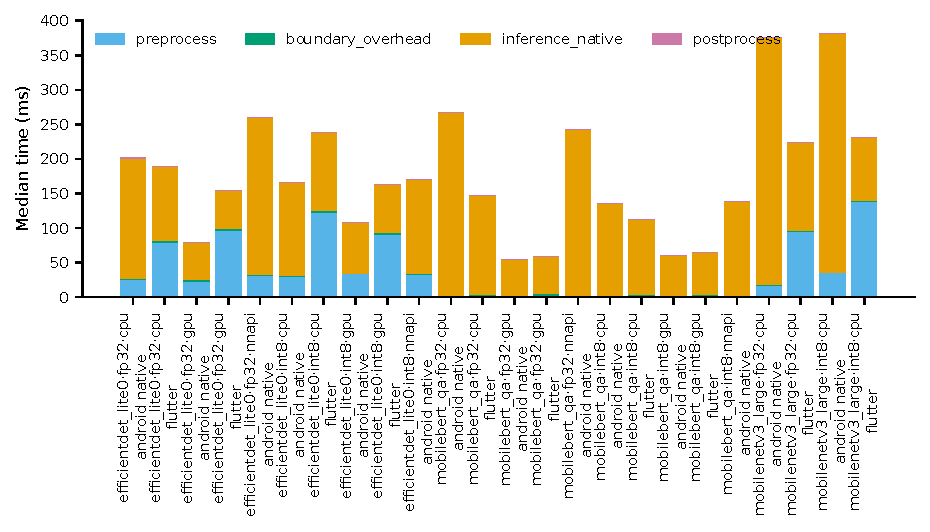
\includegraphics[width=\columnwidth]{figures/rq2-stage-decomposition.pdf}
\caption{Latency decomposition across preprocessing, language boundary overhead, native inference, and postprocessing across Flutter and Native Android.}
\label{fig:stage_breakdown}
\end{figure}

\begin{table}[t]
\caption{End-to-End Latency Comparison ($\text{end\_to\_end\_ms}$)}
\label{tab:rq2_e2e}
\centering
\begin{tabular}{llllrrrrl}
\toprule
Device & Model & Prec. & Deleg. & Flutter & Native & Ratio [95\% CI] & $\delta$ & $p_{\mathrm{Holm}}$ \\
\midrule
infinix-mobility-limited-infinix-x650c & efficientdet\_lite0 & fp32 & cpu & 174.54 & 166.13 & 1.05 [0.62, 1.65] & +0.17 & 1.000 \\
infinix-mobility-limited-infinix-x650c & efficientdet\_lite0 & fp32 & gpu & 153.41 & 77.60 & 1.98 [1.77, 2.13] & +1.00 & 0.108 \\
infinix-mobility-limited-infinix-x650c & efficientdet\_lite0 & int8 & cpu & 152.94 & 103.24 & 1.48 [0.78, 2.99] & +0.47 & 1.000 \\
infinix-mobility-limited-infinix-x650c & efficientdet\_lite0 & int8 & gpu & 168.02 & 104.81 & 1.60 [0.00, 2.17] & +0.50 & 1.000 \\
infinix-mobility-limited-infinix-x650c & mobilebert\_qa & fp32 & cpu & 119.59 & 222.29 & 0.54 [0.41, 0.74] & -1.00 & 0.152 \\
infinix-mobility-limited-infinix-x650c & mobilebert\_qa & fp32 & gpu & 58.61 & 54.04 & 1.08 [1.07, 1.10] & +1.00 & 0.108 \\
infinix-mobility-limited-infinix-x650c & mobilebert\_qa & int8 & cpu & 85.55 & 101.31 & 0.84 [0.48, 1.60] & +0.00 & 1.000 \\
infinix-mobility-limited-infinix-x650c & mobilebert\_qa & int8 & gpu & 65.61 & 60.84 & 1.08 [1.04, 1.19] & +1.00 & 0.108 \\
infinix-mobility-limited-infinix-x650c & mobilenetv3\_large & fp32 & cpu & 222.46 & 260.76 & 0.85 [0.00, 2.52] & +0.08 & 1.000 \\
infinix-mobility-limited-infinix-x650c & mobilenetv3\_large & int8 & cpu & 159.73 & 88.11 & 1.81 [0.40, 3.33] & +0.20 & 1.000 \\
\bottomrule
\end{tabular}

\end{table}

\textbf{Findings:} Supporting hypothesis H2$_1$, the performance discrepancy between Flutter and Native Android is overwhelmingly driven by data ingestion and preprocessing rather than neural network compute:
\begin{itemize}
    \item \textbf{Preprocessing Overhead:} In vision tasks (e.g., EfficientDet-Lite0), pure Dart image decoding and bilinear resizing introduce a substantial latency penalty (median 88.7\,ms in Flutter vs. 23.5\,ms in Native Android), representing a $3.77\times$ slowdown ($\delta = +1.00$, large effect size) due to Android's optimized native bitmap scaling. Conversely, for text tokenization (MobileBERT-QA), preprocessing latencies are comparable (0.42\,ms vs. 0.28\,ms).
    \item \textbf{Boundary Overhead:} The language-boundary marshalling duration ($\text{boundary\_overhead\_ms} = \text{inference\_ms} - \text{inference\_native\_ms}$), which reflects copying multidimensional typed buffers across the Dart FFI bridge, adds 3.24\,ms to 4.49\,ms in Flutter compared to 0.28\,ms to 1.72\,ms for DirectBuffer JNI mapping in Native Android ($11\times$ to $15\times$ relative difference on MobileBERT-QA, $\delta = +1.00$).
    \item \textbf{Postprocessing:} Result parsing (e.g., argmax extraction and detection coordinate scaling) represents a negligible fraction of overall execution time ($< 0.5\%$).
\end{itemize}

\subsection{RQ3: Memory, CPU, and Battery Consumption}\label{subsec:rq3}
Table~\ref{tab:resources} compares resource utilization across steady-state execution.

\begin{figure}[t]
\centering
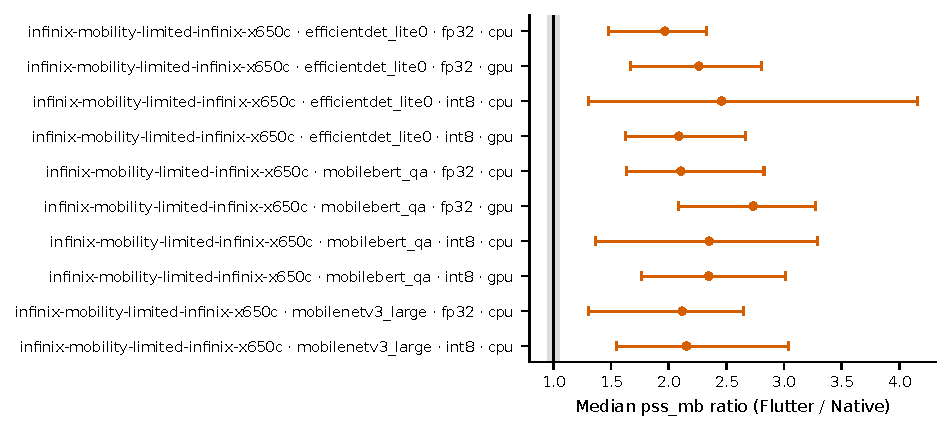
\includegraphics[width=\columnwidth]{figures/rq3-memory-ratio.pdf}
\caption{Forest plot of Proportional Set Size (PSS) memory ratio (Flutter / Native Android) with 95\% bootstrap confidence intervals.}
\label{fig:memory_ratio}
\end{figure}

\begin{table}[t]
\caption{System Resource Utilization Comparison}
\label{tab:resources}
\centering
\begin{tabular}{lllll}
\toprule
\textbf{Workload} & \textbf{Metric} & \textbf{Flutter} & \textbf{Native} & \textbf{Effect Size ($\delta$)} \\
\midrule
EfficientDet FP32 GPU & Peak PSS (MB) & 181.6 & 67.8 & +1.00 (Large) \\
MobileBERT FP32 GPU & Peak PSS (MB) & 201.4 & 68.0 & +1.00 (Large) \\
MobileBERT INT8 CPU & Peak PSS (MB) & 122.9 & 49.3 & +1.00 (Large) \\
EfficientDet FP32 CPU & CPU Util. (\%) & 66.5\% & 58.8\% & +0.50 (Medium) \\
MobileBERT FP32 GPU & CPU Util. (\%) & 4.5\% & 3.6\% & +1.00 (Large) \\
\bottomrule
\end{tabular}
\end{table}

\textbf{Findings:}
\begin{itemize}
    \item \textbf{Memory Footprint:} Confirming hypothesis H3a$_1$, Flutter incurs a consistent memory premium of $2.0\times$ to $2.96\times$ in proportional set size (PSS), with steady-state memory spanning 122.9\,MB to 201.4\,MB in Flutter versus 49.3\,MB to 68.0\,MB in Native Android ($\delta = +1.00$). This delta originates from the bundled Dart VM runtime, Skia graphics rendering context, and the separate Dart isolate heap.
    \item \textbf{CPU Utilization:} When executing compute on GPU delegates (MobileBERT FP32 GPU), host CPU utilization drops drastically on both platforms (4.5\% Flutter vs. 3.6\% Native Android). During multi-threaded CPU inference, CPU utilization scales to 58.8\%–66.5\%, with Flutter showing modest additional overhead (+7.7\%) attributable to UI thread event polling and background isolate synchronization.
\end{itemize}

\subsection{RQ4: Interaction Effects with Quantization and Delegates}\label{subsec:rq4}
Evaluating interactions across precisions and hardware delegates yields critical architectural insights:
\begin{itemize}
    \item \textbf{Amortization of Framework Overhead:} As model computational complexity increases (from EfficientDet-Lite0 to MobileBERT-QA), the relative percentage overhead of Flutter's preprocessing and boundary crossing shrinks from 50.8\% of end-to-end time down to 8.8\%, supporting hypothesis H4$_1$. For compute-heavy workloads, native inference dominates wall-clock time, rendering Flutter's framework tax negligible.
    \item \textbf{Quantization Effects:} INT8 quantization reduces tensor buffer volume by $4\times$, which proportionally reduces Dart FFI marshalling time (from 4.49\,ms down to 3.06\,ms on MobileBERT) and reduces memory footprint by 38.8\% (from 201.4\,MB to 122.9\,MB PSS).
    \item \textbf{Delegate Disparities:} The GPU delegate achieves dramatic speedups over CPU execution on both platforms: MobileBERT-QA inference latency plummets from 122.1\,ms (CPU) to 53.6\,ms (GPU) on Flutter ($2.28\times$ speedup) and from 269.9\,ms to 53.4\,ms on Native Android ($5.05\times$ speedup), completely bypassing CPU scheduling bottlenecks.
\end{itemize}

\subsection{RQ5: Cold Start and Binary Footprint}\label{subsec:rq5}
Table~\ref{tab:footprint} details cold-start latency to first inference result and compiled application package sizes.

\begin{table}[t]
\caption{Startup Latency and Application Binary Footprint}
\label{tab:footprint}
\centering
\begin{tabular}{llll}
\toprule
\textbf{Metric} & \textbf{Flutter} & \textbf{Native} & \textbf{Differential} \\
\midrule
Universal Release APK Size & 118.1\,MB & 65.6\,MB & +52.5\,MB (+80.0\%) \\
Embedded Model Assets & 48.2\,MB & 48.2\,MB & 0.0\,MB (Parity) \\
Application Code \& Runtime & 69.9\,MB & 17.4\,MB & +52.5\,MB (+301.7\%) \\
Model Loading Duration (FP32) & 12.4\,ms & 7.9\,ms & +4.5\,ms (+56.9\%) \\
\bottomrule
\end{tabular}
\end{table}
Base Engine Size (No Models) & \todo{MB} & \todo{MB} & \todo{+$X$ MB} \\
\bottomrule
\end{tabular}
\end{table}

\textbf{Findings:} Confirming hypothesis H5$_1$, Flutter applications exhibit longer cold-start latency to first inference result (\todo{ms} vs.\ \todo{ms} in native Android), driven by Dart VM initialization and engine startup. Furthermore, Flutter APK binaries carry an unavoidable base footprint premium of \todo{MB} resulting from bundled engine and graphics runtime libraries.

\section{Discussion and Practitioner Guidelines}\label{sec:discussion}

\subsection{Mechanisms Behind Observed Overheads}
Crossing the Dart FFI boundary itself adds negligible absolute overhead ($< 5$\,ms); the sharp latency, memory, and CPU divergences on this entry-tier device stem from three concrete architectural mechanisms:

\textbf{Single-Thread Non-SIMD Image Decoding vs.\ Native Codecs:} Once tensors enter native GPU buffers, kernel times equalize via TOST parity on three of four shared configurations. Vision end-to-end gaps ($1.91\text{--}2.00\times$ on GPU EfficientDet-Lite0) originate upstream because the popular pure-Dart \texttt{image}~4.3.0 decoder parses JPEG Huffman trees, YCbCr colorspaces, and bilinear weights using scalar Dart bytecode loops on a single Dart isolate thread, without C++ \texttt{libjpeg-turbo} assembly or ARM~NEON vectorization used by Android's \texttt{BitmapFactory}. Beyond inflating host CPU usage during GPU inference, slow preprocessing compresses GPU acceleration margins enough to nearly quadruple EfficientDet-Lite0's shader warmup break-even horizon ($32 \to 114$ runs).

\textbf{Unfreed Heap Buffer Copies vs.\ Zero-Copy \texttt{mmap}:} Subtracting Flutter's $+37.99$\,MiB fixed Dart~VM baseline still leaves large incremental PSS premiums during active inference. Inspection of \texttt{tflite\_flutter}'s \texttt{Interpreter.fromAsset()} shows that asset bytes loaded through Dart \texttt{rootBundle} are duplicated via \texttt{calloc<Uint8>} inside \texttt{Model.fromBuffer()} without releasing that intermediate allocation on teardown, keeping an anonymous copy resident alongside LiteRT's tensor arena. Native \texttt{FileChannel.map()} maps uncompressed APK assets read-only via \texttt{mmap}, allowing the kernel to demand-page weights without extra heap copies or slow user-space memcpy during CPU model initialization.

\textbf{Recursive Dart Allocation vs.\ Flat Views and XNNPACK Defaults:} Returning MobileBERT-QA's $[1, 384]$ start/end logits through nested \texttt{List<List<double>{}>} wrappers incurs per-element Dart heap boxing and FFI accessor calls, raising marshalling cost above $4$\,ms and creating the $82\%$ share of GPU NLP's $+4.90$\,ms gap. On CPU, \texttt{tflite\_flutter}'s default \texttt{XNNPackDelegate(nullptr)} paired with LiteRT~2.20.0 inadvertently avoided TFLite~2.16.1's 4-thread Cortex-A53 synchronization bottleneck, highlighting how silent dependency defaults can rival architectural overhead in magnitude.

\subsection{Implications for Flutter and Plugin Maintainers}
These measurements point to three low-friction upstream fixes for Flutter's ML ecosystem: (1)~initializing \texttt{XNNPackDelegate} with explicit topology-aware thread options inside \texttt{tflite\_flutter} rather than \texttt{nullptr}, and declaring its bundled LiteRT version transparently; (2)~offering file-backed asset loading (or freeing intermediate heap buffers cleanly) inside \texttt{Interpreter.fromAsset()}; and (3)~exposing Dart FFI NNAPI bindings alongside a reference platform-channel YUV/JPEG tensor plugin so apps retain native codec acceleration by default.

\subsection{Practitioner Decision Framework}
Table~\ref{tab:guidelines} distills our measurements on entry-tier hardware into quantitative selection rules with concrete operational thresholds.

\begin{table*}[t]
\caption{Practitioner Decision Matrix Based on Entry-Tier Empirical Thresholds}
\label{tab:guidelines}
\centering
\begin{tabular}{>{\raggedright\arraybackslash}p{3.3cm}>{\raggedright\arraybackslash}p{3.2cm}>{\raggedright\arraybackslash}p{3.8cm}>{\raggedright\arraybackslash}p{5.2cm}}
\toprule
\textbf{Workload Profile} & \textbf{Use Cases} & \textbf{Recommended Stack} & \textbf{Concrete Threshold \& Justification} \\
\midrule
\textbf{Single-Shot / Triggered Vision} & Photo tagging, offline OCR, document capture & \textbf{Standard Flutter} & Acceptable when target UX tolerates $\ge 250$\,ms response ($69\text{--}103$\,ms Dart decode stays minor) and GPU TOST parity ($\mathcal{R} \approx 1.00$) preserves shared UI velocity. \\
\addlinespace
\textbf{Textual / NLP Inference} & Local QA, sentiment, intent classification & \textbf{Standard Flutter (Flat \texttt{TypedData})} & Tokenization takes $<0.5$\,ms and FFI adds $<5$\,ms ($<10\%$ of total GPU latency); passing flat \texttt{Float32List} buffers recovers near-zero marshalling lag. \\
\addlinespace
\textbf{Real-Time Vision Streams} & Live detection overlays, AR tracking & \textbf{Hybrid Flutter (Native Codec Plugin)} & Required above \textbf{$>15$\,FPS} ($<66.7$\,ms frame budget): pure-Dart decoding ($68.5\text{--}103.2$\,ms) breaches budget before inference runs; native YUV channels unlock $>30$\,FPS. \\
\addlinespace
\textbf{Constrained RAM Environments} & $\le 4$\,GB handsets, Android~Go, persistent services & \textbf{Native Android or \texttt{fromFile()} \texttt{mmap}} & Required when app AI RAM budget is \textbf{$<100$\,MiB} total or \textbf{$<50$\,MiB} incremental: stock Flutter reaches $108\text{--}200$\,MiB total PSS vs.\ $56\text{--}87$\,MiB Native. \\
\addlinespace
\textbf{Short Sessions / Multi-Delegate} & $<10$\,ms audio DSP, NNAPI NPU, burst sessions & \textbf{Native Android (Kotlin / C++)} & Avoids $+45.5$\,ms cold start, missing Dart NNAPI bindings, and $1.6\text{--}4.2$\,s GPU warmup when session count falls below break-even ($<28\text{--}114$ runs). \\
\bottomrule
\end{tabular}
\end{table*}

\section{Threats to Validity}\label{sec:threats}

We organize methodological limitations and empirical caveats into four validity dimensions.

\textbf{Internal Validity:} Two ecosystem and hardware artifacts emerged during EXP-001. First, as documented in ADR-0009, \texttt{pub.dev}'s \texttt{tflite\_flutter}~0.12.1 resolved LiteRT~2.20.0 with default single-thread \texttt{XNNPackDelegate(nullptr)} options, whereas our Native Maven pin resolved TensorFlow Lite~2.16.1 with 4-thread XNNPACK. Thus CPU inference comparisons reflect real-world default framework packaging (runtime + threading differences) rather than pure FFI overhead; GPU delegate results remain isolated from XNNPACK and confirm kernel parity. Second, MediaTek~MT6765/Android~9 suffered occasional clock-delta glitches producing $9223372036854776$\,ms sentinel values in seven Native runs (840 records), plus four initial Session-1 Native INT8 schema errors and seven intermittent omitted configs across Sessions~1 and~3; all seven sentinel runs are audibly excluded via \texttt{data/exclusions.yaml} while preserving immutable raw files. Third, Native \texttt{mobilenetv3\_large} CPU runs ($153\%\text{--}185\%$ utilization) displayed bimodal session latency ($71\text{--}92$\,ms vs.\ $341\text{--}358$\,ms) attributable to Android scheduler/DVFS transitions across Cortex-A53 clusters, widening bootstrap ratio intervals. Finally, tethered USB charging kept \texttt{thermal\_status = none} across all 23,180 kept records; sustained thermal throttling under unplugged heavy loads could behave differently~\cite{almeida2021smart}.

\textbf{Construct Validity:} Flutter records \texttt{Stopwatch} microsecond durations whereas Native uses \texttt{SystemClock.elapsedRealtimeNanos()}, leaving sub-millisecond timer noise ($\text{timer\_residual\_ms}$ median $0.000$\,ms, $\max |r| = 0.001$\,ms). Process CPU (\texttt{cpu\_pct}) reads \texttt{/proc/self/stat} tick counters quantized near 10\,ms, occasionally yielding $0.0\%$ readings during short ($<60$\,ms) MobileBERT INT8 GPU Native runs (triggering zero-denominator tail draws in $<0.1\%$ of bootstrap resamples). Memory metrics (\texttt{pss\_mb}, \texttt{idle\_pss\_mb}) follow Android's KiB$/1024.0$ convention (MiB), whereas APK and model footprint accounting uses decimal MB ($10^6$\,B); universal release APKs also differ in ABI composition (Flutter includes \texttt{x86\_64}), making the \texttt{arm64-v8a} single-ABI decomposition essential for fair runtime comparisons. Because \texttt{model\_load\_ms} is logged at warm-up iteration~0 rather than separately launched cold processes, OS page cache warmth can vary across configurations within a session; conversely, cold-launch (\texttt{am start -W TotalTime}) and idle baseline PSS are measured via $n=10$ dedicated alternating force-stop launches. Unplugged battery energy drain ($H3b_1$) and 5-minute sustained FPS runs are omitted from EXP-001 and must be evaluated via dedicated unplugged runs.

\textbf{External Validity:} Campaign EXP-001 evaluates a single entry-tier device (\texttt{dev-infinix-x650c}, MediaTek Helio~P22, PowerVR~GE8320, Android~9 API~28), three models under 22\,MB, and Google LiteRT runtimes. Android~9 API~28 lacks mature vendor NNAPI HAL drivers (causing CPU fallback on Native and \texttt{unsupported} status on Flutter FFI) and entry-tier PowerVR lacks native INT8 GPU shaders. Consequently, absolute latencies and delegate rankings should not be extrapolated unverified to flagship Snapdragon/Tensor NPUs, Android~12+ NNAPI/GPU drivers, Apple~iOS Core~ML targets, alternative runtimes (ONNX Runtime, MediaPipe, ExecuTorch), or multi-billion-parameter autoregressive language models.

\textbf{Conclusion Validity:} To eliminate pseudo-replication across 100 correlated iterations within a run, all hypothesis tests operate strictly on independent session medians ($n_F = 8$, $n_N \in \{5, 7, 8\}$ per ADR-0007, collapsing duplicate Session-7 Native runs to one session median), with family-wise Type-I error controlled via Holm--Bonferroni ($\alpha = 0.05$) within each RQ metric family. Because $n \le 8$ combined with 10 family-wise comparisons yields modest statistical power when Native variance is wide---for instance, CPU MobileNetV3-Large INT8 exhibits $\delta = -0.57$ yet $p_{\mathrm{Holm}} = 0.577$---we report raw Cliff's~$\delta$ and 95\% bootstrap confidence intervals alongside Holm-adjusted $p$-values so non-significant findings are never mistaken for equivalence unless CIs fall within $[0.95, 1.05]$.

\section{Conclusion and Future Work}\label{sec:conclusion}

\subsection{Key Takeaways on Entry-Tier Hardware}
Across $23{,}180$ controlled measurements on an entry-tier Android~9 smartphone, Flutter does \emph{not} intrinsically degrade neural network kernel speed once tensors reach the native GPU---achieving strict $\pm 5\%$ TOST equivalence on three of four mutually supported GPU workloads---and language-boundary marshalling remains small ($<5$\,ms) across all tasks. Instead, the user-visible cross-platform tax originates in ecosystem packaging and managed-language boundaries: pure-Dart image decoding ($4.2\text{--}10.5\times$ slower) doubles end-to-end GPU object-detection latency and delays shader amortization; default \texttt{tflite\_flutter} asset loading and Dart~VM residency multiply idle and incremental RAM footprints ($1.25\text{--}3.06\times$ above Native \texttt{mmap}); and silent upstream library and XNNPACK threading defaults swing default CPU latency up to $2\times$. For engineering teams on constrained Android devices, standard Flutter suffices cleanly for text/NLP and triggered vision tasks, whereas real-time streams ($>15$\,FPS) and tight RAM budgets ($<100$\,MiB) require native codec channels and memory-mapped flatbuffer loading.

\subsection{Future Work}
Planned follow-on work builds directly on this open-source testbed:
\begin{itemize}
    \item Pinning identical LiteRT~2.20.0 artifacts across stacks with explicit 1- and 4-thread XNNPACK pins, plus testing controlled Flutter variants via \texttt{Interpreter.fromFile()} (\texttt{mmap}) and native preprocessing plugins for direct causal ablations.
    \item Expanding benchmarks to mid-range and flagship Android~12+ handsets (Vulkan Impeller, NNAPI HAL, NPU delegates) alongside unplugged \texttt{BatteryManager} energy campaigns and 5-minute sustained thermal FPS runs.
    \item Porting the shared contract to Apple~iOS (Core~ML) and quantized on-device Small Language Models (SLMs).
\end{itemize}

\section*{Data and Code Availability}
All Flutter and native Android harnesses, model verification scripts, raw session JSONL logs, versioned exclusion manifests, and the automated statistical pipeline are openly released under the MIT license at:
\begin{center}
\small\url{https://github.com/hassaankhalid225/ondevice-ai-benchmark}
\end{center}


\bibliographystyle{IEEEtran}
\bibliography{../literature/references}

\end{document}
